\section{Mean, variance and effect}
Considering some dataset, it might at times be useful 
to do statistical analysis on some dataset to see
if it mean values are reasonable in accordance with
the theoretically predicted data.\

it might also be useful for determining if some data
set is pure noice of if it might contain some statistically
significant event.

The mean value of a dataset is given by the simple equation

\begin{align}
  \label{mean}
  \mu = \frac{1}{N}\sum_{i=0}^{N} x_{i}
\end{align}

which comes out to 5062 using matlabs sum and length functions.
Nothing interesting can be said for the mean value by itself 
but the standard deviation and variance might give some clues
as to how much the data deviates from the mean.\

both the standard deviation, $\sigma$ and the variance $\sigma^2$
are defined in the following ways

\begin{align}
  \label{eq:stdAndVar}
  \sigma &= \sqrt{\frac{1}{N}\sum_{i=0}^{N}(X_{i} - \mu)^2}\\
  \sigma^2 &= \frac{1}{N}\sum_{i=0}^{N}(X_{i} - \mu)^2
\end{align}

For both the standard deviation and the variance, using matlabs std and var
functions we get $\sigma = 38.4$ and $\sigma^2 = 1.480$. The statistical significance
of these figures however are unclear in the context of looking for exoplanets as 
is the case with this worked upon dataset.

Taking a look at the signals effect which is defined similarly to the variance

\begin{align}
  \label{eq:effect}
  s_{effect} = \frac{1}{N}\sum_{i=0}^N X_{i}^2
\end{align}

the effect of the signal is defined as the mean square of the dataset.
When we compare \eqref{eq:effect} and \eqref{eq:stdAndVar} we can see
that the variance tells us the mean distance that the signals effect has
to from the mean value of the signal.

lastly we can plot the amplitude of the dataset as a histogram to get an
idea of the most commonly occuring signal amplitudes.

\newpage

\begin{figure}[h]
  \centering
  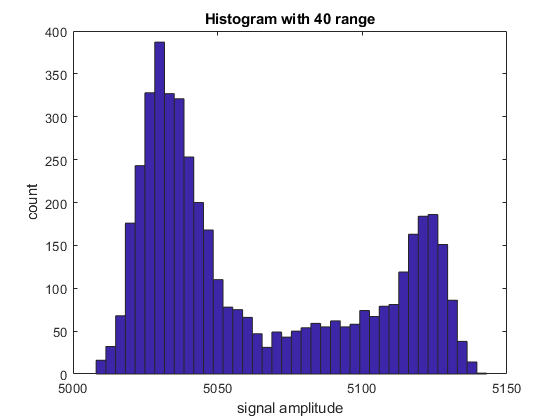
\includegraphics[width=\textwidth]{matlabstuff/amplitudeHistogram.png}
  \caption{amplitude histogram, for dataset of exoplanets}%
  \label{fig:amplitudeHistogram}
\end{figure}

\newpage
